% Define colors
\definecolor{headerColor}{HTML}{4F81BD}
\definecolor{rowColor1}{HTML}{B8CCE4}
\definecolor{rowColor2}{HTML}{DCE6F1}
\definecolor{textColor}{HTML}{000000}
\definecolor{highlightColor}{HTML}{00B0F0}
\section{Comparsion} 
\label{sec:3_6_comparsion}

In this section, we undertake a critical comparison of closely related works addressing the challenges of imbalanced multiclass streams \ref{sec:3_6_1_related_work_imbalanced}, the emergence of new classes \ref{sec:3_6_2_related_work_emergence}, and the integration of transfer learning \ref{sec:3_6_2_related_work_transfer} within streaming environments. The increasing complexity of real-world data streams necessitates advanced methodologies that can effectively manage the intricacies of these challenges. By examining various approaches in the literature, we aim to highlight their contributions, strengths, and limitations in dealing with imbalanced data distributions, adapting to new class occurrences, and leveraging transfer learning techniques. This comparative analysis not only sheds light on the current state of research but also underscores the specific gaps and unresolved issues that our work seeks to address, ultimately paving the way for more robust and adaptive solutions in the realm of streaming data classification.


\subsection{Imbalanced Stream}
\label{sec:3_6_1_related_work_imbalanced}

In the context of multi-class classification, addressing class imbalances is crucial. Multi-Label SMOTE (MLSMOTE) extends the principles of SMOTE to generate synthetic examples for each minority class label, thereby enhancing classifier performance by considering neighboring examples in the feature space. Recently, Multi-Label Synthetic Oversampling based on Local label imbalance (MLSOL) has emerged as a more effective technique. MLSOL systematically addresses local imbalances by employing distinct sampling strategies for each label. Empirical research demonstrates that MLSOL outperforms existing methods, including MLSMOTE, in terms of classification accuracy and computational efficiency. By generating synthetic samples exclusively from minority class instances within a restricted neighborhood, MLSOL produces a more compact and efficient synthetic dataset, mitigating concerns related to overfitting.
As illustrated in Fig. \ref{fig:mlsmote_mlsol}, MLSOL is more likely to select x1 as a seed instance because it is surrounded by more neighbors of the opposite class for l3. MLSMOTE assigns the label vector [0,1,0] to all synthetic instances based on their neighbors. In contrast, MLSOL creates more diverse instances by assigning labels according to their location. Moreover, synthetic instances c2 and c3 generated by MLSMOTE introduce noise, whereas MLSOL copies the labels of the nearest instance to the new examples. In summary, MLSMOTE tends to generate new instances biased toward the dominant class in the local area, whereas MLSOL effectively explores and exploits both the feature and label space.
\begin{figure*}[!ht]

    \begin{center}
      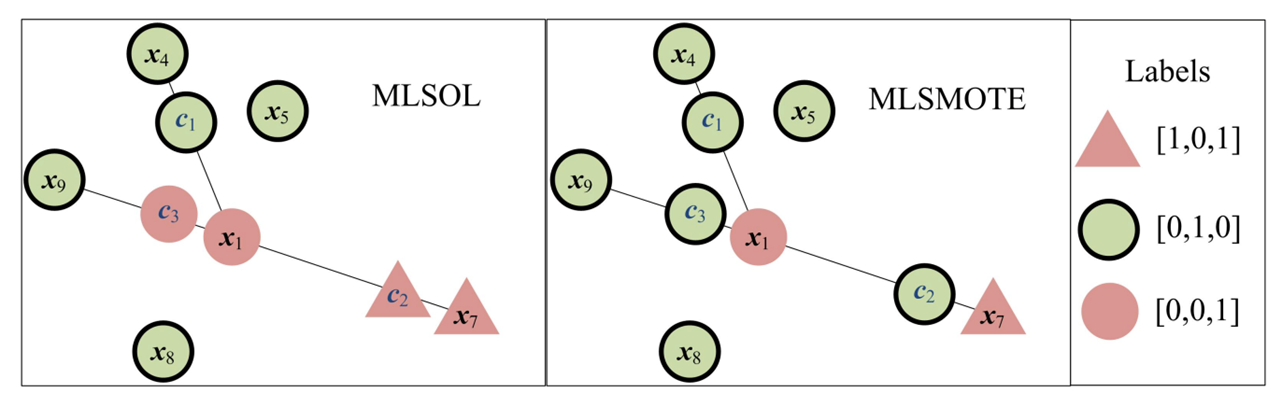
\includegraphics[width=1\textwidth]{3_State-of-the-art/fig/mlsmote_mlsol.png}
    \end{center}

    \caption{Distribution of prediction accuracy. \\ \textcolor{gray}{\fontsize{10}{0}\selectfont DOI: 110.1016/j.patcog.2021.108294}}
    \label{fig:mlsmote_mlsol}

    \end{figure*}
    
Table \ref{table:imbalanced}  presents a comparison of two methods, MLSMOTE and MLSOL, which are designed to address the issue of imbalanced data in multi-class classification. MLSMOTE enhances classifier performance by generating synthetic examples for each minority class label, thereby balancing the class distribution. Its primary advantage is the generation of these synthetic examples, which helps mitigate the imbalance. However, it has significant limitations: the synthetic samples generated might be related to the majority class, which can blur the distinction between classes, and the method struggles with overlapping classes, leading to potential misclassification. On the other hand, MLSOL systematically combats local imbalances by employing distinct sampling strategies for each label within a restricted neighborhood. This localized approach allows MLSOL to generate synthetic examples more precisely, addressing local imbalances effectively. Nonetheless, like MLSMOTE, MLSOL faces challenges with overlapping classes, which can result in misclassification in areas where class boundaries are not clear. Despite its advantages in handling local imbalances, the overlapping class issue remains a critical limitation for both methods, affecting their overall effectiveness in classification tasks.
\begin{table*}[!ht]

    \centering
    \caption{Comparison of the MLSMOTE and MLSOL methods.}
    \label{table:imbalanced}

    \small % Reduce font size
    \renewcommand{\arraystretch}{1} % Reduce cell padding
    \setlength{\tabcolsep}{4pt} % Reduce cell padding
    \setlength{\arrayrulewidth}{0.15mm}

    \begin{tabularx}{\textwidth}{|>{\centering\arraybackslash\bfseries}p{2cm}|
                                       >{\raggedright\arraybackslash}X|
                                       >{\raggedright\arraybackslash}X|
                                       >{\raggedright\arraybackslash}X|}
    \hline
    \textbf{Method} & \textbf{Theory} & \textbf{Advantages} & \textbf{Limitations} \\ 
    \hline
    \textbf{MLSMOTE} & 
    MLSMOTE significantly enhances classifier performance by generating synthetic examples for each minority class label. & 
    Generating synthetic examples for each minority class label. & 
    \begin{itemize}[leftmargin=*]
        \item Random synthetic samples may be related to the majority class.
        \item Overlapping classes.
    \end{itemize} \\ 
    \hline
    \textbf{MLSOL} & 
    MLSOL systematically combats local imbalances within the domain of multi-class classification by employing distinct sampling strategies for each label. & 
    Generating synthetic examples for each minority class label within a restricted neighborhood. & 
    \begin{itemize}[leftmargin=*]
        \item Overlapping classes.
    \end{itemize} \\
    \hline
    \end{tabularx}
    \end{table*}










\subsection{Emergence of new classes}
\label{sec:3_6_2_related_work_emergence}


Effectively detecting and adapting to new classes in streaming data is crucial for maintaining classification accuracy. Tree-based methods like SENCForest and SEEN utilize anomaly detection but face high false positive rates and runtime inefficiencies. SENNE improves detection performance using a nearest neighbor ensemble but suffers from longer runtimes due to the lack of an effective model retirement mechanism. The k-nearest Neighbor Ensemble-based method (KNNENS) addresses new class detection and known class classification using a k-nearest neighbor-based hypersphere ensemble and dynamic model updates. However, a critical limitation of these methods is their inadequate handling of concept drift, which is essential for detecting new classes and retraining the classification model. These methods represent the best closely related work for our proposal, which aims to build upon them by incorporating robust concept drift techniques for more adaptive and resilient classification systems.

Fig. \ref{fig:SENCForest} illustrates the SENCForest approach, which divides the space into three regions (normal, outlying, and anomaly) and detects emerging new classes (anomalies) using a calculated threshold path length. Fig. \ref{fig:SENNE} depicts the SENNE algorithm, where hyperplanes are drawn in three dimensions (x1, x2, and x3) for each class (Fig. \ref{fig:SENNE}a). New instances are then classified as emerging or known classes based on the rank of each class (Fig. \ref{fig:SENNE}b). Fig. \ref{fig:KENNE} presents the KNNENS algorithm, which draws hyperplanes for all class samples (Fig. \ref{fig:KENNE}a), and classifies new instances using a voting mechanism to determine if the instance is an emerging or known class (Fig. \ref{fig:KENNE}b). These visualizations highlight the operational differences between the SENNE and KNNENS algorithms in handling the classification of emerging and known classes.

\begin{figure*}[!ht]
    \centering
    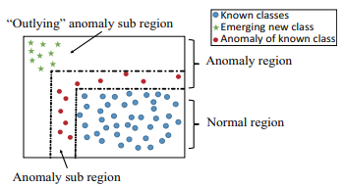
\includegraphics[width=0.85\textwidth]{3_State-of-the-art/fig/SENCForst.png}
    \caption{Overview of stream emerging new classes. \\
    \textcolor{gray}{\fontsize{10}{0}\selectfont DOI: 10.1109/TKDE.2017.2691702}}
    \label{fig:SENCForest}
\end{figure*}
    

\begin{figure*}[!ht]
    \begin{center}
        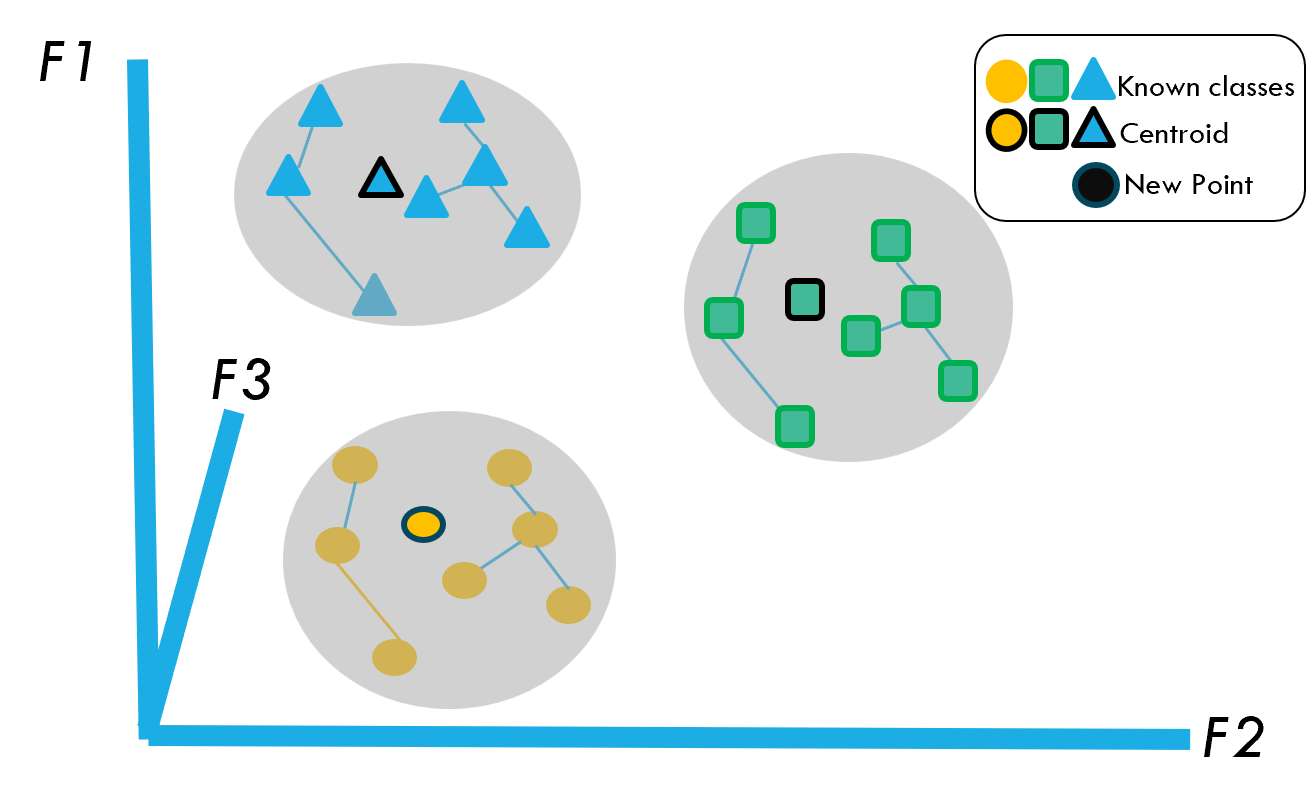
\includegraphics[width=.49\textwidth]{3_State-of-the-art/fig/senne0.png} 
        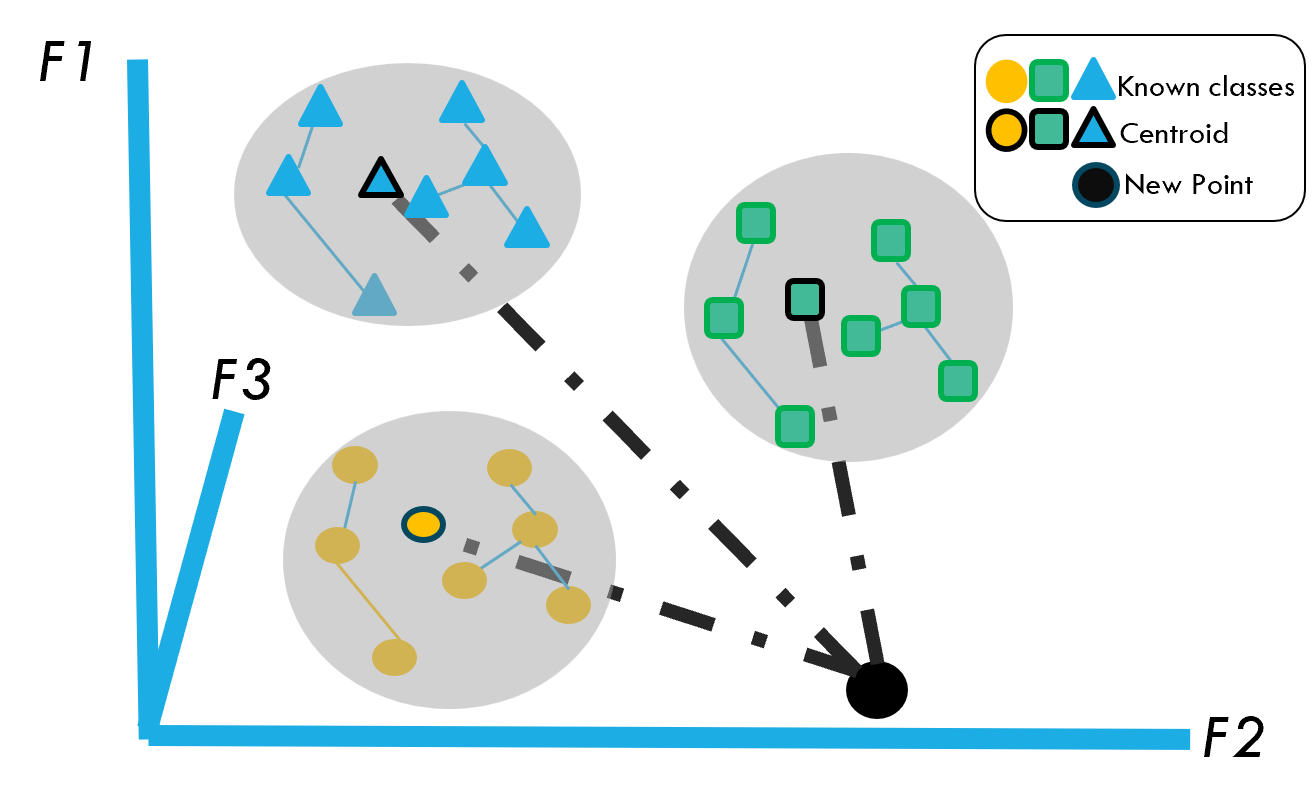
\includegraphics[width=.49\textwidth]{3_State-of-the-art/fig/senne.png} 
        (a)\hspace{6.5cm}(b)
    \end{center}
    \caption{Overview of the Stream Emerging Nearest Neighbor Ensemble (SENNE).}
    \label{fig:SENNE}
    \end{figure*}
    \vline
    \begin{figure*}[!ht]    
        \begin{center}
            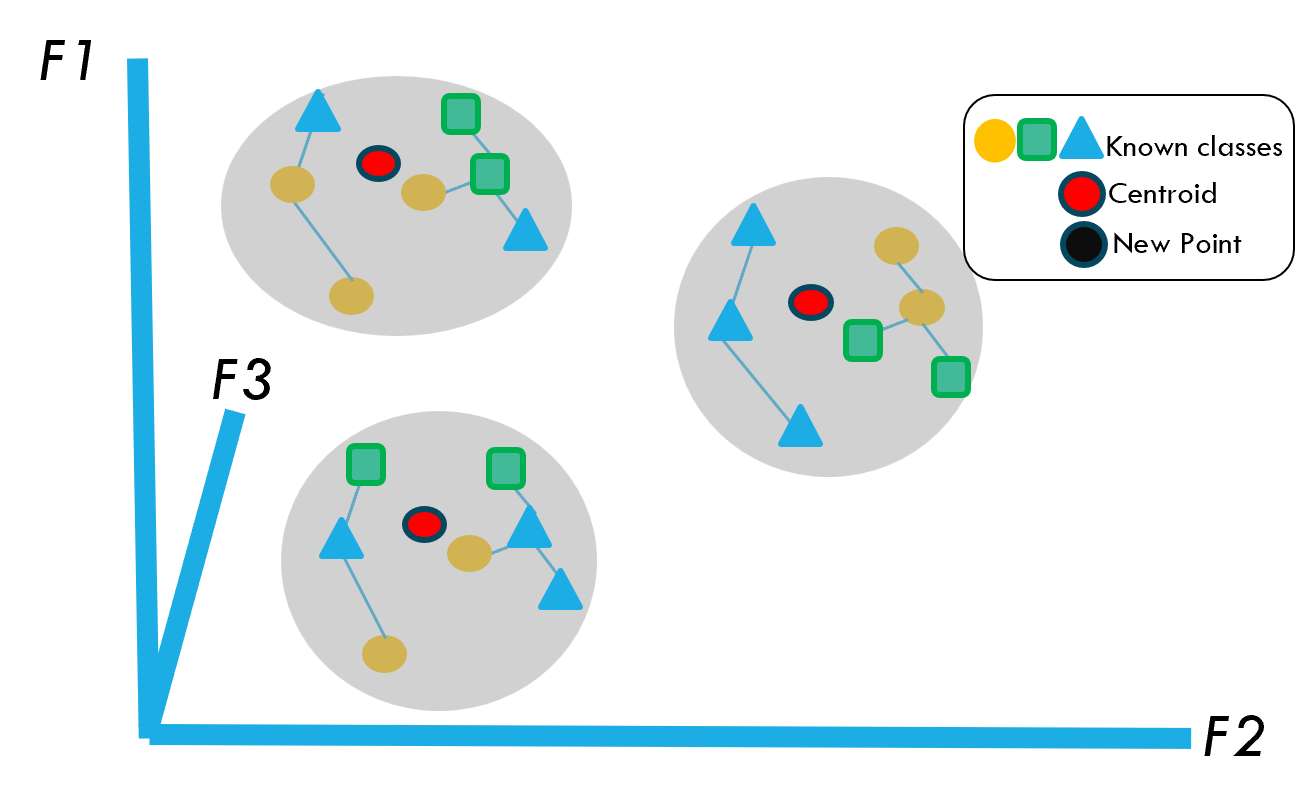
\includegraphics[width=.49\textwidth]{3_State-of-the-art/fig/kenne0.png} 
            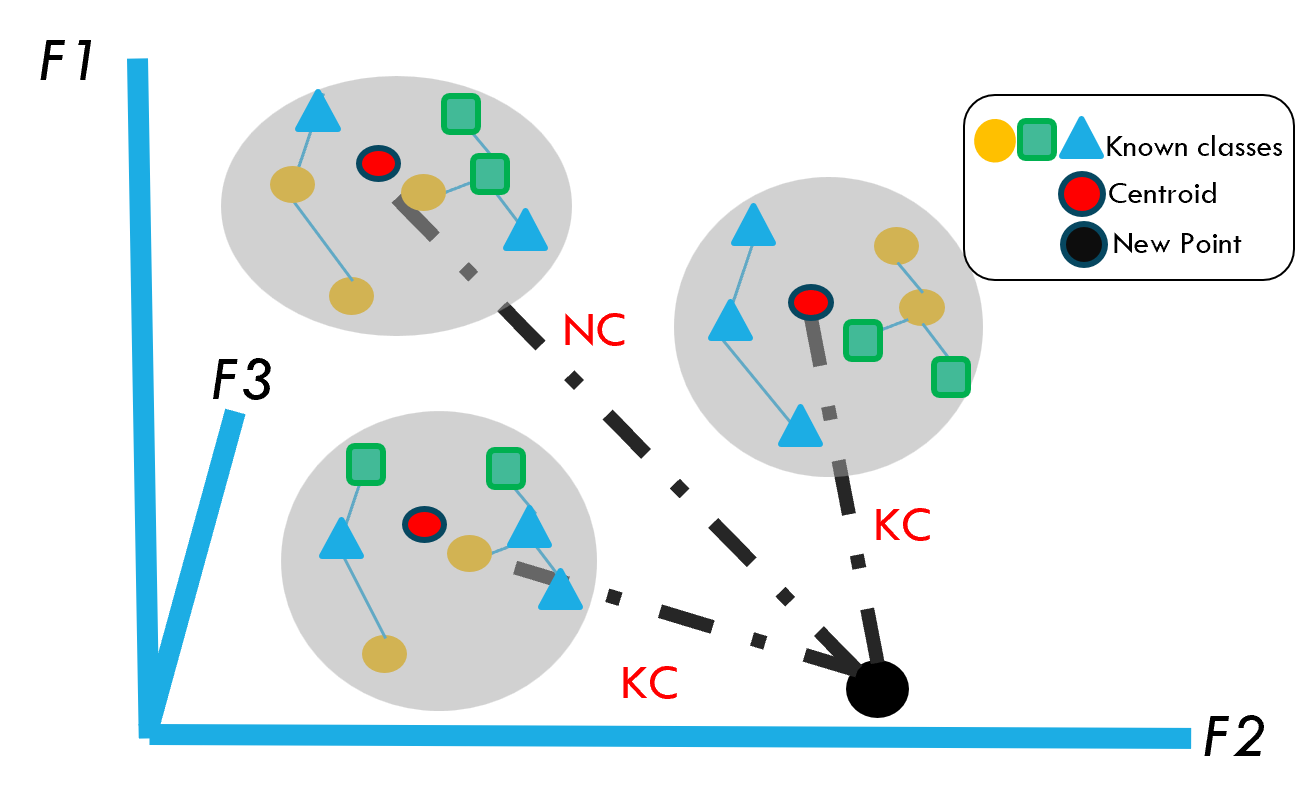
\includegraphics[width=.49\textwidth]{3_State-of-the-art/fig/kenne.png}
            (a)\hspace{6.5cm}(b)
            \end{center}
    
        \caption{Overview of the k-nearest Neighbor Ensemble-based (KENNE).}
        \label{fig:KENNE}
        \end{figure*}
        

        Table\ref{table:emerging} compares three methods for emerging class detection: SENCForest, SENNE, and KNNENS. SENCForest employs the anomaly detection method iForest for new class detection and uses a threshold path to identify anomalies, serving both as an unsupervised anomaly detector and a supervised classifier. However, it has a high potential for false positives and depends on a complex path length threshold. SENNE utilizes a nearest neighbor-based hypersphere of one class ensemble to explore local neighborhood information and sort distances, handling both low and high geometric distances between classes. Its limitations include the assumption that the distribution of known classes remains unchanged and it has lengthy update times. KNNENS employs a nearest neighbor-based hypersphere of all class ensembles to explore local neighborhood information, reducing false positives for new classes without needing true labels for model updates. However, like SENNE, it assumes that the distribution of known classes remains unchanged.

\begin{table*}[!ht]

    \centering
    \caption{Comparison of the SENCForest, SENNE, and KENNE methods.}
    \label{table:emerging}
    \small % Reduce font size
    \renewcommand{\arraystretch}{1} % Reduce cell padding
    \setlength{\tabcolsep}{4pt} % Reduce cell padding
    \setlength{\arrayrulewidth}{0.15mm}
    \begin{tabularx}{\textwidth}{|>{\centering\arraybackslash\bfseries}p{2cm}|
                                       >{\raggedright\arraybackslash}X|
                                       >{\raggedright\arraybackslash}X|
                                       >{\raggedright\arraybackslash}X|}
    \hline
    \textbf{Method} & \textbf{Theory} & \textbf{Advantages} & \textbf{Limitations} \\ 
    \hline
    \textbf{SENCForst} & 
    employs anomaly detection method iForest \cite{wang2010negative} for a new class detection and then applies threshold path to detect the anomalies. & 
    SENCForest serves as both an unsupervised anomaly detector and a supervised classifier.&
    \begin{itemize}[leftmargin=*]
        \item Potential for High False Positives.
        \item Dependency on Path Length Threshold (more complexity).
    \end{itemize} \\ 
    \hline
    \textbf{SENNE} & 
    nearest neighbor-based hypersphere of one class ensemble to explore local neighborhood information and sort distance to calculate distance. & 
    SENNE is able to handle both the low and high geometric distance between two classes in the feature space. & 
    \begin{itemize}[leftmargin=*]
        \item Assumes that the distribution of known classes remains unchanged.
        \item Take long time for update.
    \end{itemize} \\ 
    \hline
    \textbf{KENNE} & 
    nearest neighbor-based hypersphere of all class ensemble to explore local neighborhood information. & 
    KNNENS to reduce false positives for the new class. KNNENS does not require true labels to update the model. & 
    \begin{itemize}[leftmargin=*]
        \item Assumes that the distribution of known classes remains unchanged.
    \end{itemize} \\
    \hline
    \end{tabularx}
    \end{table*}













\subsection{Transfer Learning}
\label{sec:3_6_2_related_work_transfer}

In the realm of transfer learning, three prominent methods—CORAL, Melanie, and HE-CDTL—serve as closely related approaches to our proposed method. Correlation Alignment (CORAL) is an asymmetric transformation approach that aligns sub-space bases using second-order statistics. By employing a learned transformation matrix, CORAL projects source instances into the target domain, thereby minimizing domain discrepancies and reducing negative knowledge transfer. Melanie addresses the challenge of non-stationary environments through an online ensemble learning approach. It incrementally trains models from both source and target domains, dynamically adjusting their weights to handle concept drift, and combines these models via a weighted-sum approach as shown in Fig. \ref{coral_fig}. As Shown in Fig. \ref{cdtl_fig} This method can be extended to Concept Drift Transfer Learning (CDTL) by using an ensemble for chunk-based concept drift. HE-CDTL, designed explicitly for CDTL, leverages knowledge from source domains and historical time steps within the target domain to enhance learning performance. It utilizes a class-wise weighted ensemble for historical knowledge and implements AW-CORAL for extracting knowledge from source domains. The class-wise weighted ensemble allows individual classes to select historical knowledge independently, while AW-CORAL minimizes domain disparities and mitigates negative knowledge transfer. Extensive experiments have shown HE-CDTL to outperform baseline methods in addressing transfer learning challenges in the context of concept drift. Together, these methods provide a comprehensive framework for effective transfer learning in dynamic and evolving data environments.

Table\ref{table:transfer} compares three methods: CORAL, Melanie, and HE-CDTL. CORAL (Correlation Alignment) utilizes a learned transformation matrix and Singular Value Decomposition (SVD) to project source instances into the target domain, effectively minimizing domain discrepancy and reducing negative knowledge transfer. However, it faces challenges with non-stationary and heterogeneous data. Melanie (Multisource Online Transfer learning for Non-stationary Environments) addresses online learning problems where data in source and target domains are generated from non-stationary environments. Its advantages include considering online problems but it too is limited by the complexities of online learning and data heterogeneity. HE-CDTL (Class-wise Weighted and Domain-wise Ensemble) minimizes domain shift by aligning second-order statistics of source and target distributions, leveraging historical knowledge to reduce disparities between domains. Despite its strengths, it relies on the quality of the source domain and also struggles with heterogeneous data.
\begin{figure*}[!ht]

    \begin{center}
        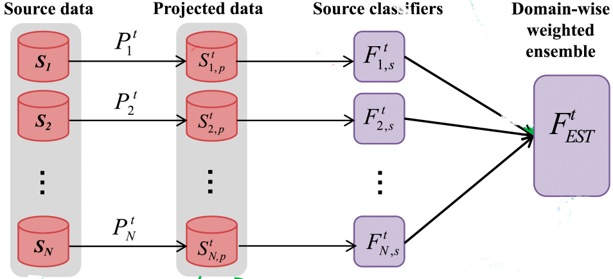
\includegraphics[width=.85\textwidth]{3_State-of-the-art/fig/coral.png} 
    \end{center}
    \caption{Overview of CORrelation ALignment (CORAL)}
    \label{coral_fig}
    \end{figure*}
    \begin{figure*}[!ht]    
        \begin{center}
            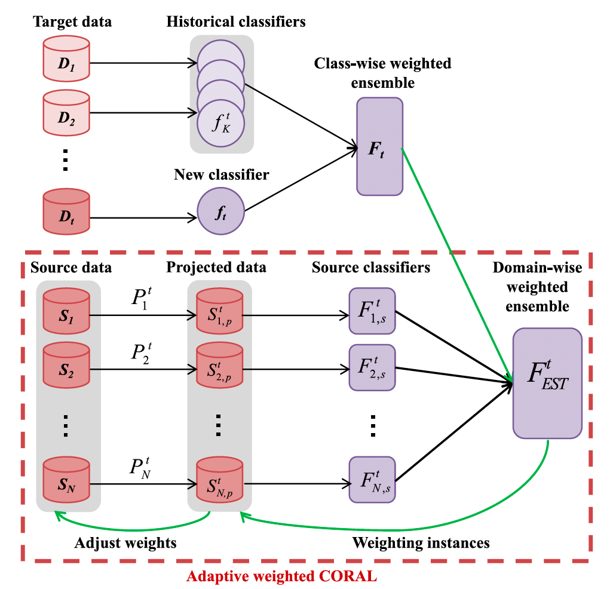
\includegraphics[width=.85\textwidth]{3_State-of-the-art/fig/cdtl.png} 
        \end{center}
        \caption{Overview of Concept Drift Transfer Learning (CDTL).}
        \label{cdtl_fig}

        \end{figure*}

\begin{table*}[!ht]
    \centering
    \caption{Comparison of the CORAL, Malanie, and CDTL methods.}
    \label{table:transfer}
    \small % Reduce font size
    \renewcommand{\arraystretch}{1} % Reduce cell padding
    \setlength{\tabcolsep}{4pt} % Reduce cell padding
    \setlength{\arrayrulewidth}{0.15mm}
    \begin{tabularx}{\textwidth}{|>{\centering\arraybackslash\bfseries}p{2cm}|
                                       >{\raggedright\arraybackslash}X|
                                       >{\raggedright\arraybackslash}X|
                                       >{\raggedright\arraybackslash}X|}
    \hline
    \textbf{Method} & \textbf{Theory} & \textbf{Advantages} & \textbf{Limitations} \\ 
    \hline
    \textbf{CORAL} & 
    Correlation Alignment (CORAL) uses a learned transformation matrix and Singular Value Decomposition (SVD)  to project the source instances into the target domain. & 
    CORAL can minimize domain discrepancy across
source and target domains, meanwhile reducing the negative
knowledge transfer. & 
    \begin{itemize}[leftmargin=*]
        \item Non-stationary environments.
        \item Heterogenous multisource.
    \end{itemize} \\ 
    \hline
    \textbf{Melanie} & 
    Multi-sourcE onLine TrAnsfer
learning for Non-statIonary Environments (Melanie). utilize the class-wise weighted . & 
It considers
an online problem in which the data in source and target
domains are generated from non-stationary environments. & 
    \begin{itemize}[leftmargin=*]
        \item Online Learning based only.
        \item Heterogenous multisource.
    \end{itemize} \\
    \hline
    \textbf{MLSOL} & 
    HE-CDTL uses the class-wise weighted and domain wise ensemble for historical knowledge and reduce the disparities between the source and target domains . & 
    HE-CDTL minimizes domain shift by aligning the second-order statistics of source and target distributions. & 
    \begin{itemize}[leftmargin=*]
        \item Depend on Source Domain Quality.
        \item Heterogenous multisource.
    \end{itemize} \\
    \hline
    \end{tabularx}
    \end{table*}
